\fakesection{Unsupervised Learning and Large Scale Problems}{\hfill\small\texttt{/src/session\_3.m}, \texttt{/src/homework\_3.m}}

\fakesubsection{Kernel principal component analysis}{}

The point of \textit{linear principal component analysis (PCA)} is to find a linear transformation (a projection onto an orthogonal basis) such that the variance of the projected data points is maximised. It's an old method introduced by Pearson. The transformed variables are called principal components. By disregarding some of these it is possible to achieve a dimensionality reduction while still capturing most of the important information carried by the input data. This can be used for denoising purposes.

\begin{figure}[h]
\centering
%
\subfloat[De-noising with linear PCA.]{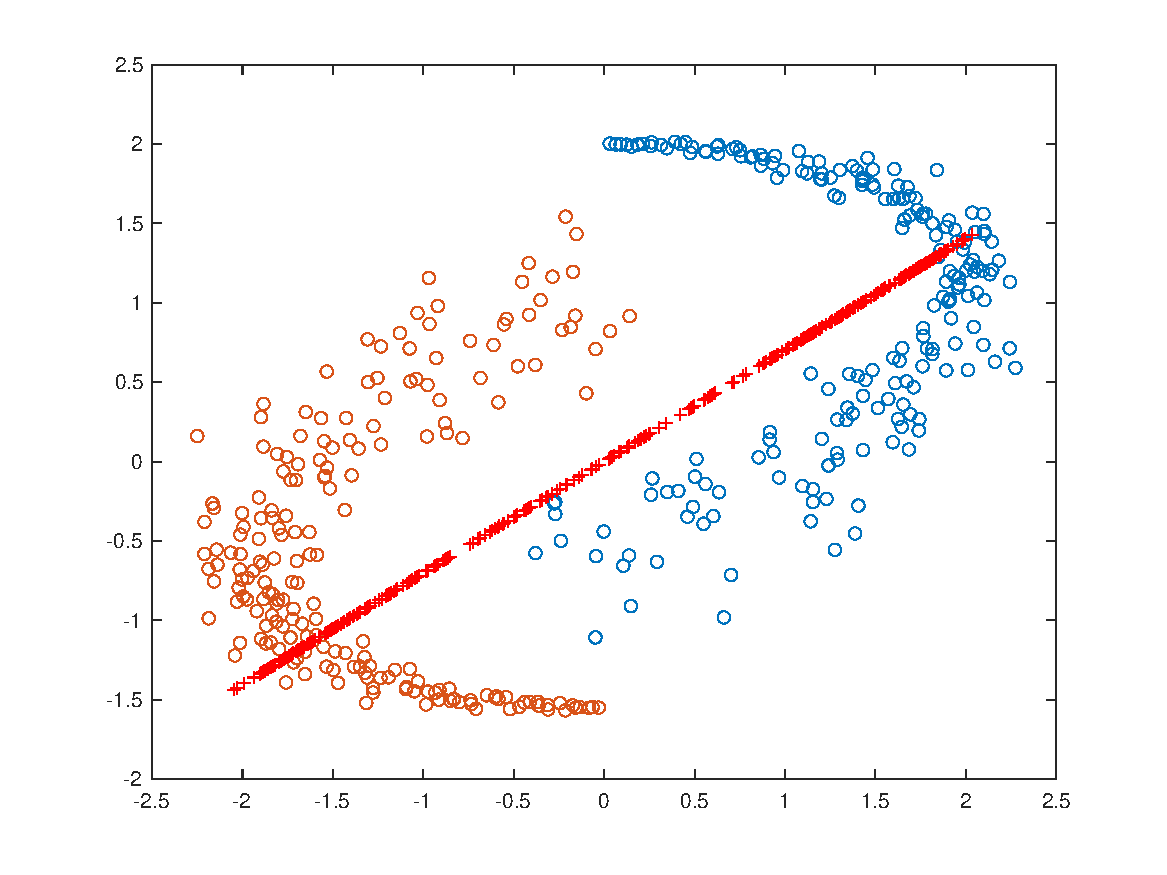
\includegraphics[width=0.35\textwidth]{../src/figures/kpca/linear}}\\
%
\subfloat[$\sigma^2=0.4,n_h=2$.]{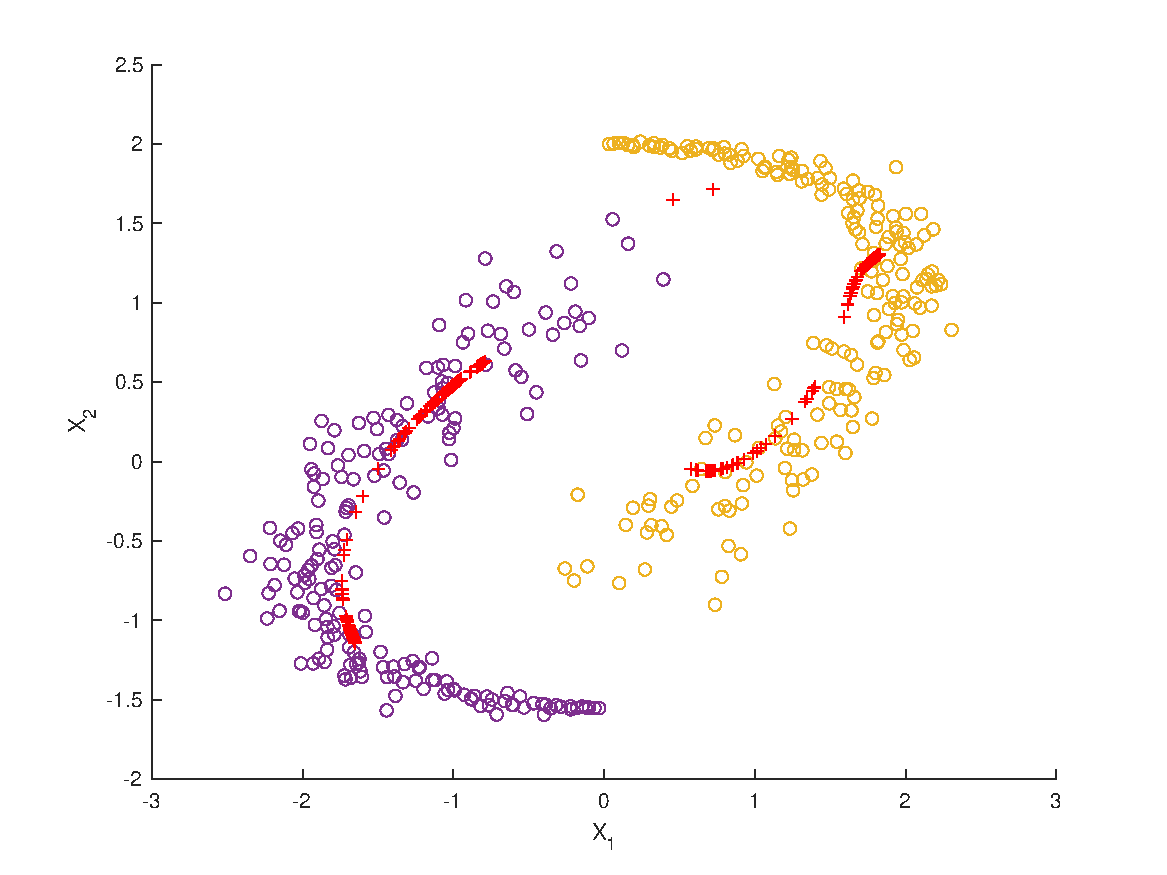
\includegraphics[width=0.25\textwidth]{../src/figures/kpca/kpca_2}}\quad
\subfloat[$\sigma^2=0.4,n_h=6$.]{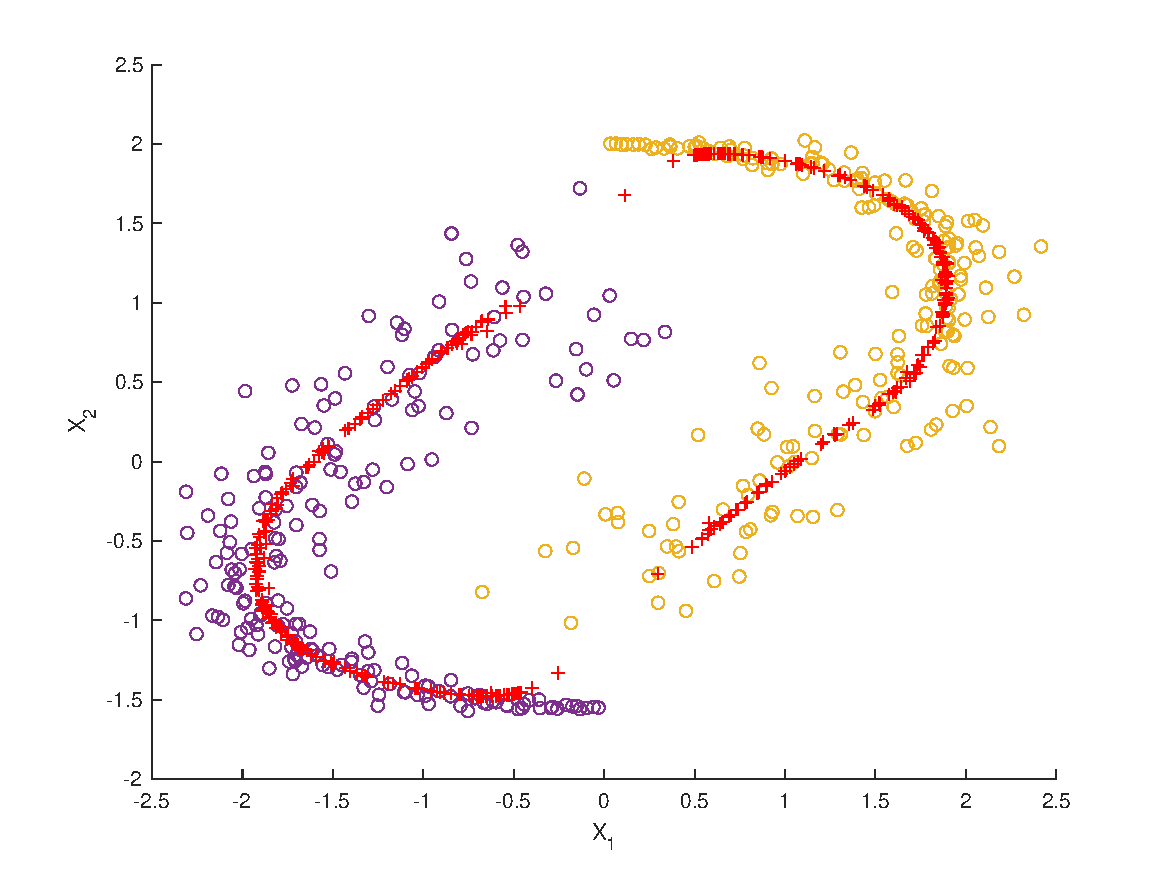
\includegraphics[width=0.25\textwidth]{../src/figures/kpca/kpca_6}}\quad
\subfloat[$\sigma^2=0.4,n_h=20$.]{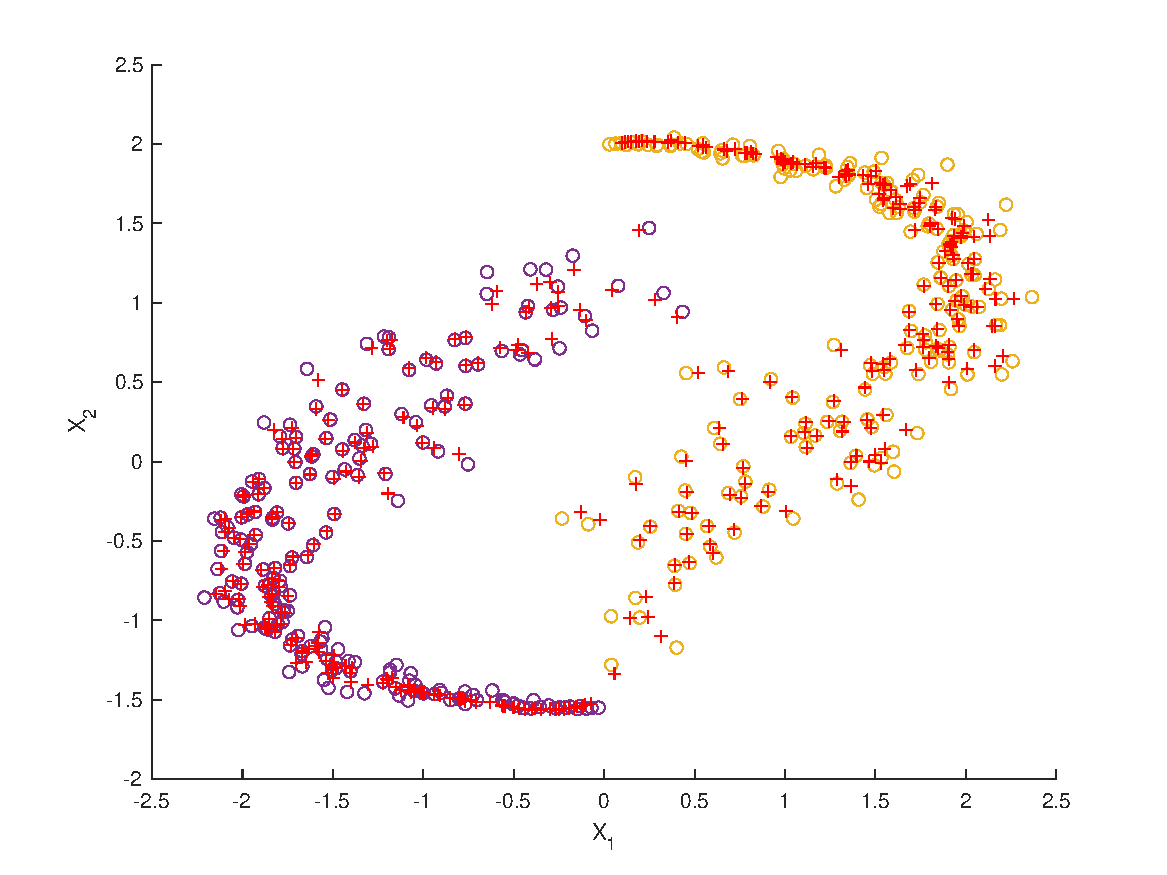
\includegraphics[width=0.25\textwidth]{../src/figures/kpca/kpca_20}}\\
%
\subfloat[$\sigma^2=1.0,n_h=2$.]{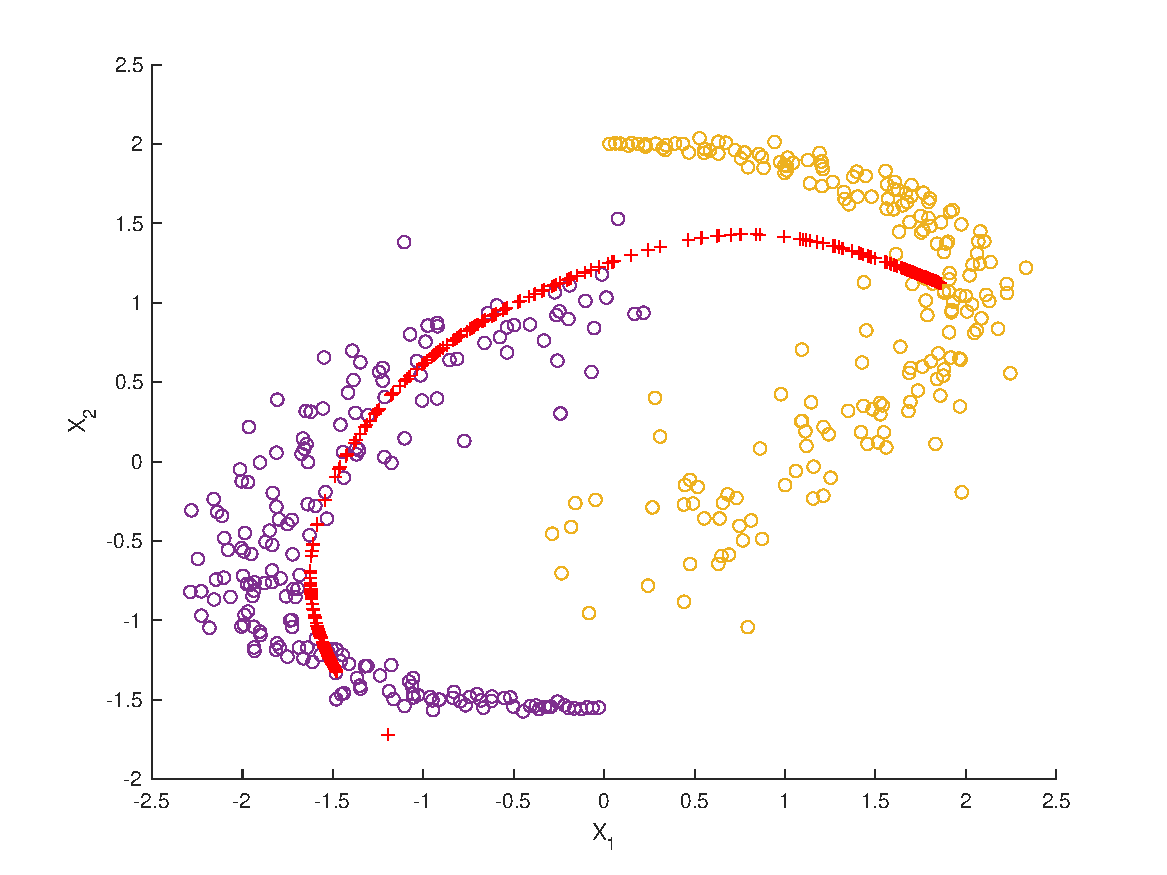
\includegraphics[width=0.25\textwidth]{../src/figures/kpca/kpca_bis_2}}\quad
\subfloat[$\sigma^2=1.0,n_h=6$.]{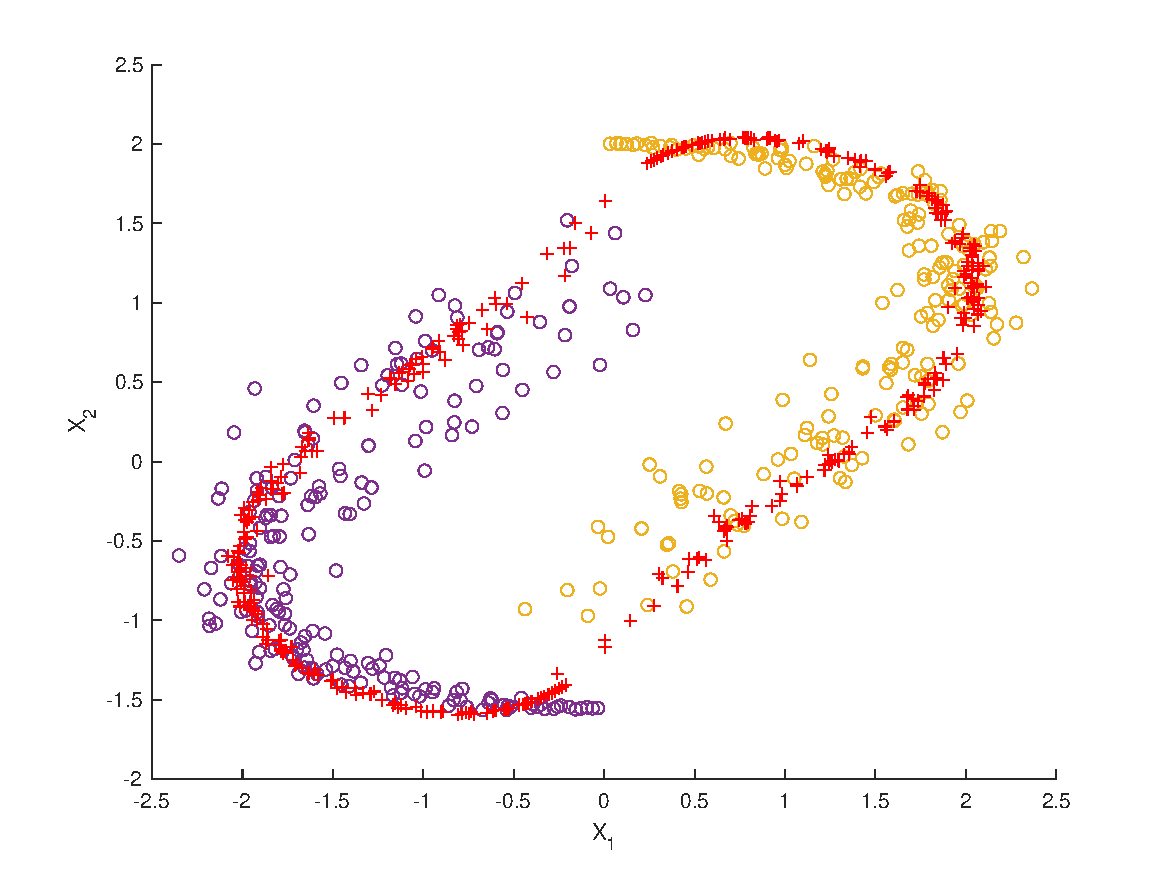
\includegraphics[width=0.25\textwidth]{../src/figures/kpca/kpca_bis_6}}\quad
\subfloat[$\sigma^2=1.0,n_h=20$.]{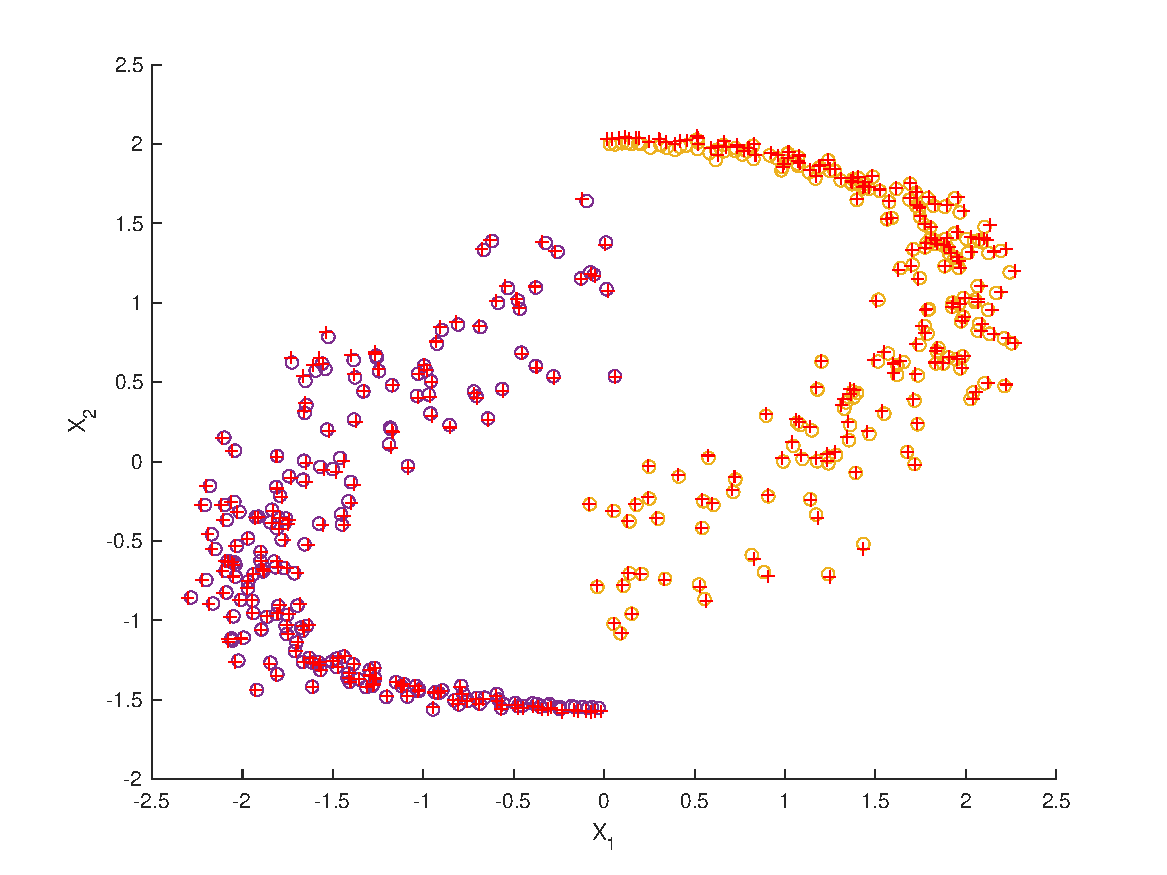
\includegraphics[width=0.25\textwidth]{../src/figures/kpca/kpca_bis_20}}\\
%
\subfloat[$\sigma^2=10.0,n_h=2$.]{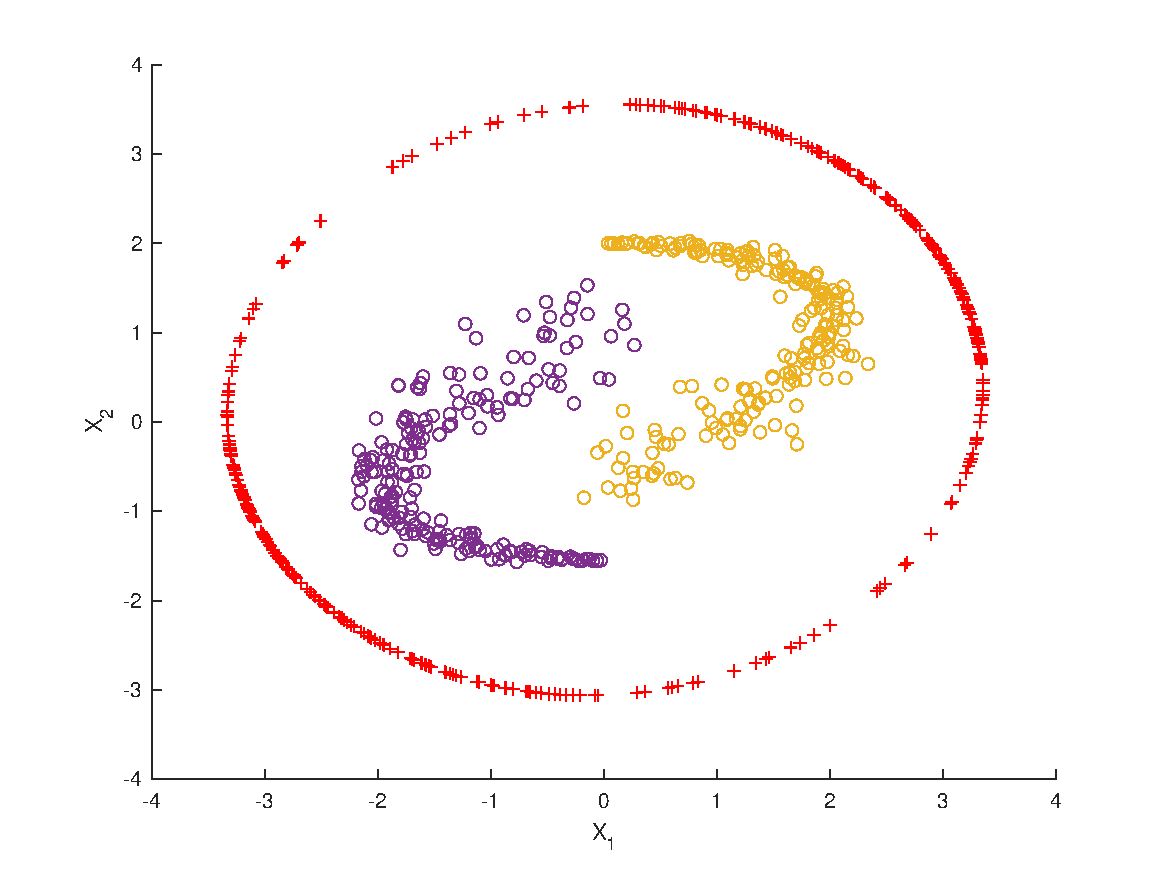
\includegraphics[width=0.25\textwidth]{../src/figures/kpca/kpca_tris_2}}\quad
\subfloat[$\sigma^2=10.0,n_h=6$.]{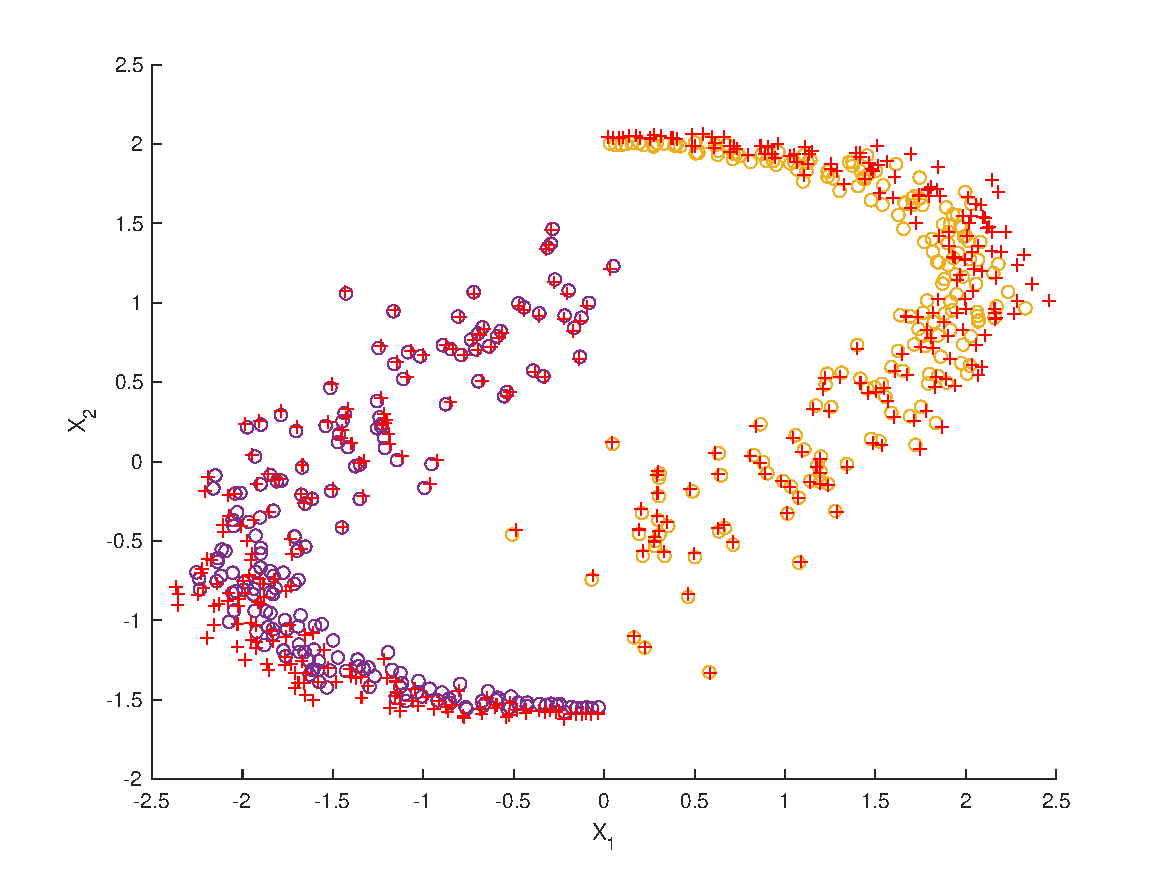
\includegraphics[width=0.25\textwidth]{../src/figures/kpca/kpca_tris_6}}\quad
\subfloat[$\sigma^2=10.0,n_h=20$.]{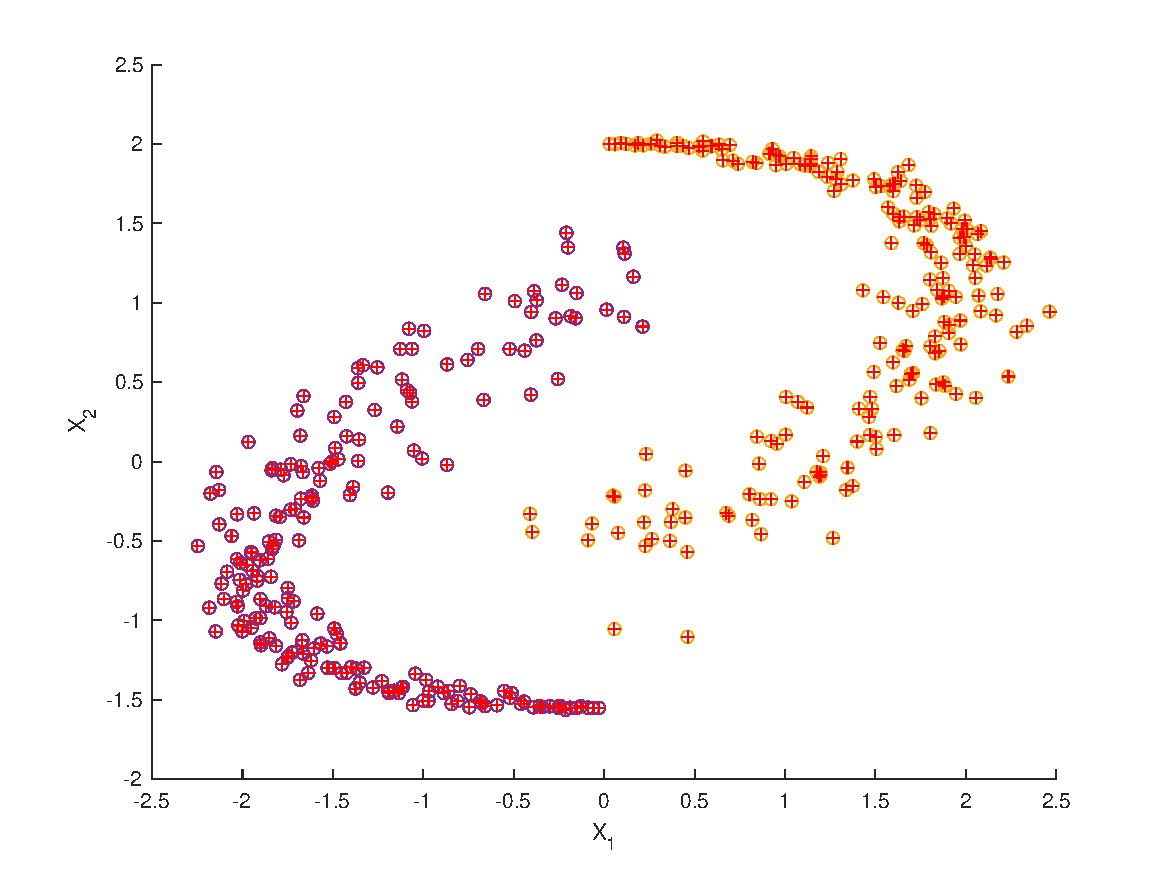
\includegraphics[width=0.25\textwidth]{../src/figures/kpca/kpca_tris_20}}\\
%
\caption{De-noising a toy dataset consisting of two spirals. The number of data points equals 400, the data point dispersion 0.3. $n_h$ is the number of components. Retaining too few principal components leads to a poor result while retaining too many of them prevents any de-noising.}
\label{kpcatoy}
\end{figure}

\par Like \textit{Fisher discriminant analysis (FDA)} it is possible to relate this to LS-SVMs and formulate it as a constraint optimisation problem :
$$\max_{w,e}\quad\mathcal{J}_P(w,e)=\gamma\frac{1}{2}\sum_{k=1}^Ne_k^2-\frac{1}{2}w^Tw\qquad\text{such that $e_k=w^T\cdot x_k\quad(k=1,\dots, N)$}$$
Here too, a dual form can be introduced using Lagrange multipliers. This makes it possible to apply the kernel trick which can make for a non-linear approach (in which case PCA is applied in the feature space). Additionally an increase in the number of dimensions becomes possible when the number of training samples is larger than the number of dimensions. The bias term is responsible for centering the kernel matrix automatically rather than having to do this beforehand. This is especially interesting in the case of \textit{kernel spectral clustering (KSC)} which is considered in the next paragraph and where centring is not a straightforward thing to do.

\par Because the alternative PCA formulation is model-based it becomes possible to do so-called out-of-sample extensions - the solution is not limited to the input data. It also becomes possible to tune models and find the right parameters that fit the data. However, because of the unsupervised nature of PCA this is not trivial. If the resulting model is meant to be used as a sort of preprocessing step e.g. for use in classification or in the context of a reconstruction problem (assuming an information bottleneck) then tuning can be done on the basis of the related loss function by making use of validation sets (as demonstrated previously). Otherwise it is possible to use common cross-validation techniques for linear PCA to pick an appropriate number of components followed by cross-validation based on pre-images to find useful values of the kernel parameters. These pre-images are approximations of inverse transformations of kernel PCA outputs back to the input space and can be used to calculate the reconstruction error for any point in the validation set (which consists of one data point in the case of LOOCV).

\par As an example of this method, consider the de-noising of a toy dataset the result of which are shown in figure \ref{kpcatoy}. Tuning is done manually. When the number of principal components increases the reconstruction improves which is not surprising. More meaningfully, retaining a smaller number of principal components results in good de-noising performance. As per usual the linear approach (classical PCA) is not able to capture the non-linearities in the input data leading to poor results for this particular dataset. The $\sigma^2$ parameter in the Gaussian kernel can lead to a loss of non-noisy information when set too low (or a lack of de-noising if set too high, as seen in figure \ref{kpcatoy}).

\fakesubsection{Spectral clustering}{}

Classification problems were considered in the first section of this report. In a classification setting a model is constructed which is made to predict what class some data point belongs to. These models are trained in a supervised way i.e. there's an annotated training set and test set which are used to determine appropriate parameters for the model and for evaluating it. In a clustering setting the number of classes $k$ is not necessarily set beforehand but can be tuned. A model is trained in an unsupervised manner such that it clusters data points on the basis of some similarity measure. 

\begin{figure}[h]
\centering
%
\subfloat[$\sigma^2=0.001$.]{
\begin{minipage}{0.48\textwidth}
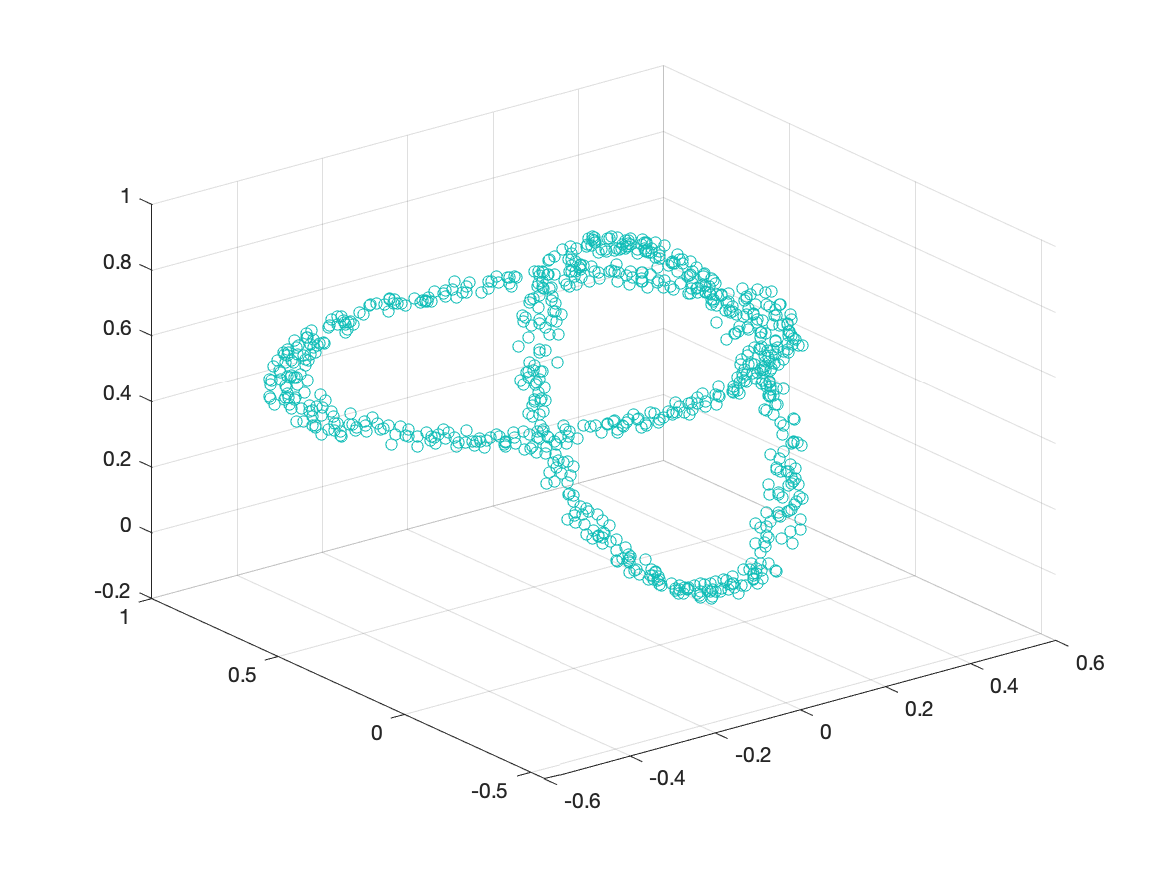
\includegraphics[width=0.45\textwidth]{../src/figures/spectral/rings_clusters_1}

\includegraphics[width=0.4\textwidth]{../src/figures/spectral/rings_block_1}
\end{minipage}}\quad
\subfloat[$\sigma^2=0.005$.]{
\begin{minipage}{0.48\textwidth}
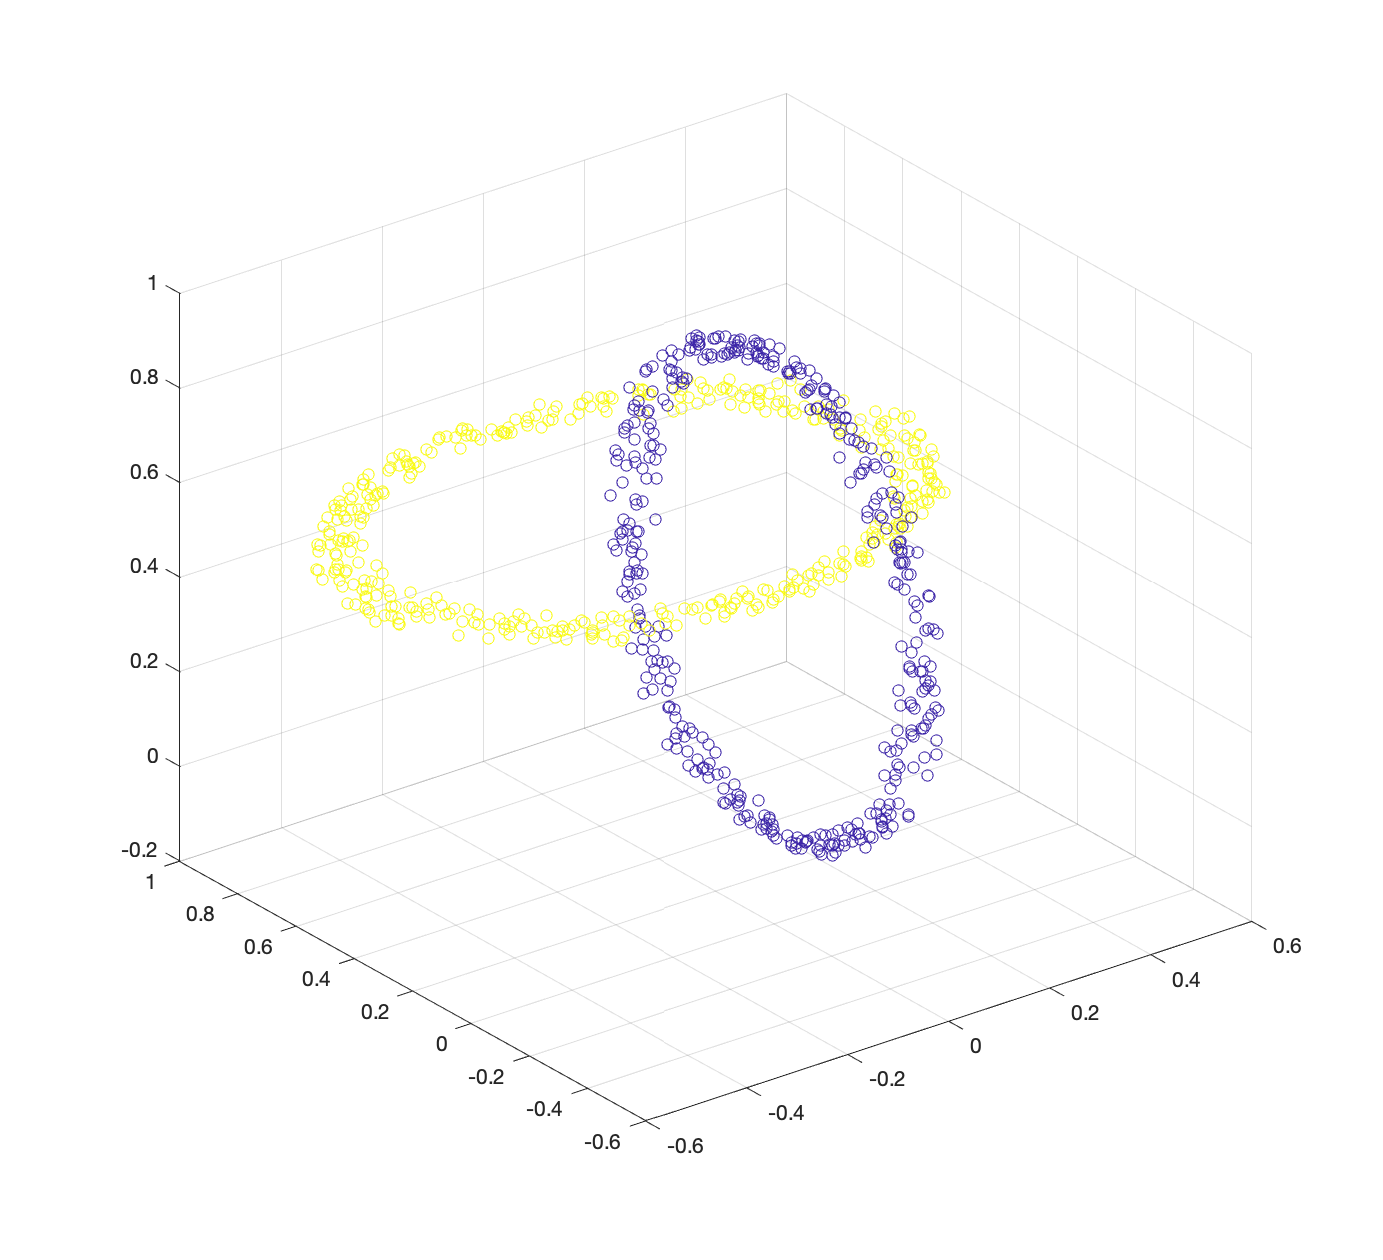
\includegraphics[width=0.45\textwidth]{../src/figures/spectral/rings_clusters_5}
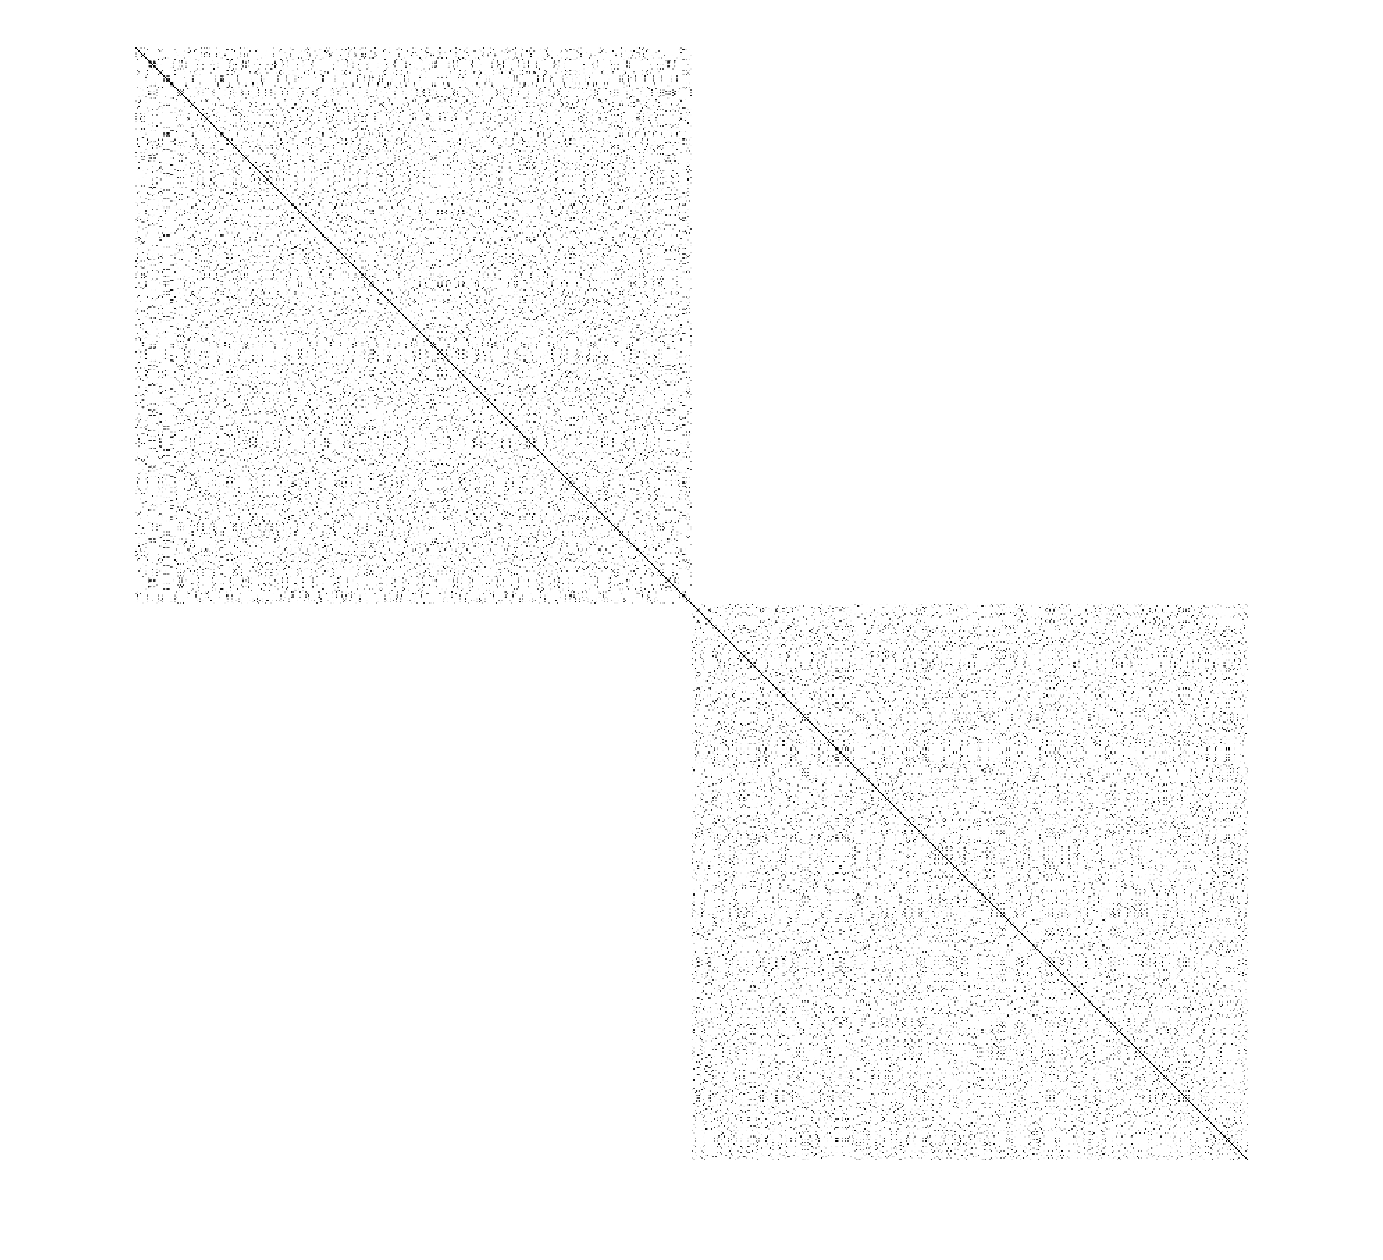
\includegraphics[width=0.4\textwidth]{../src/figures/spectral/rings_block_5}
\end{minipage}}\\
%
\subfloat[$\sigma^2=0.01$.]{
\begin{minipage}{0.48\textwidth}
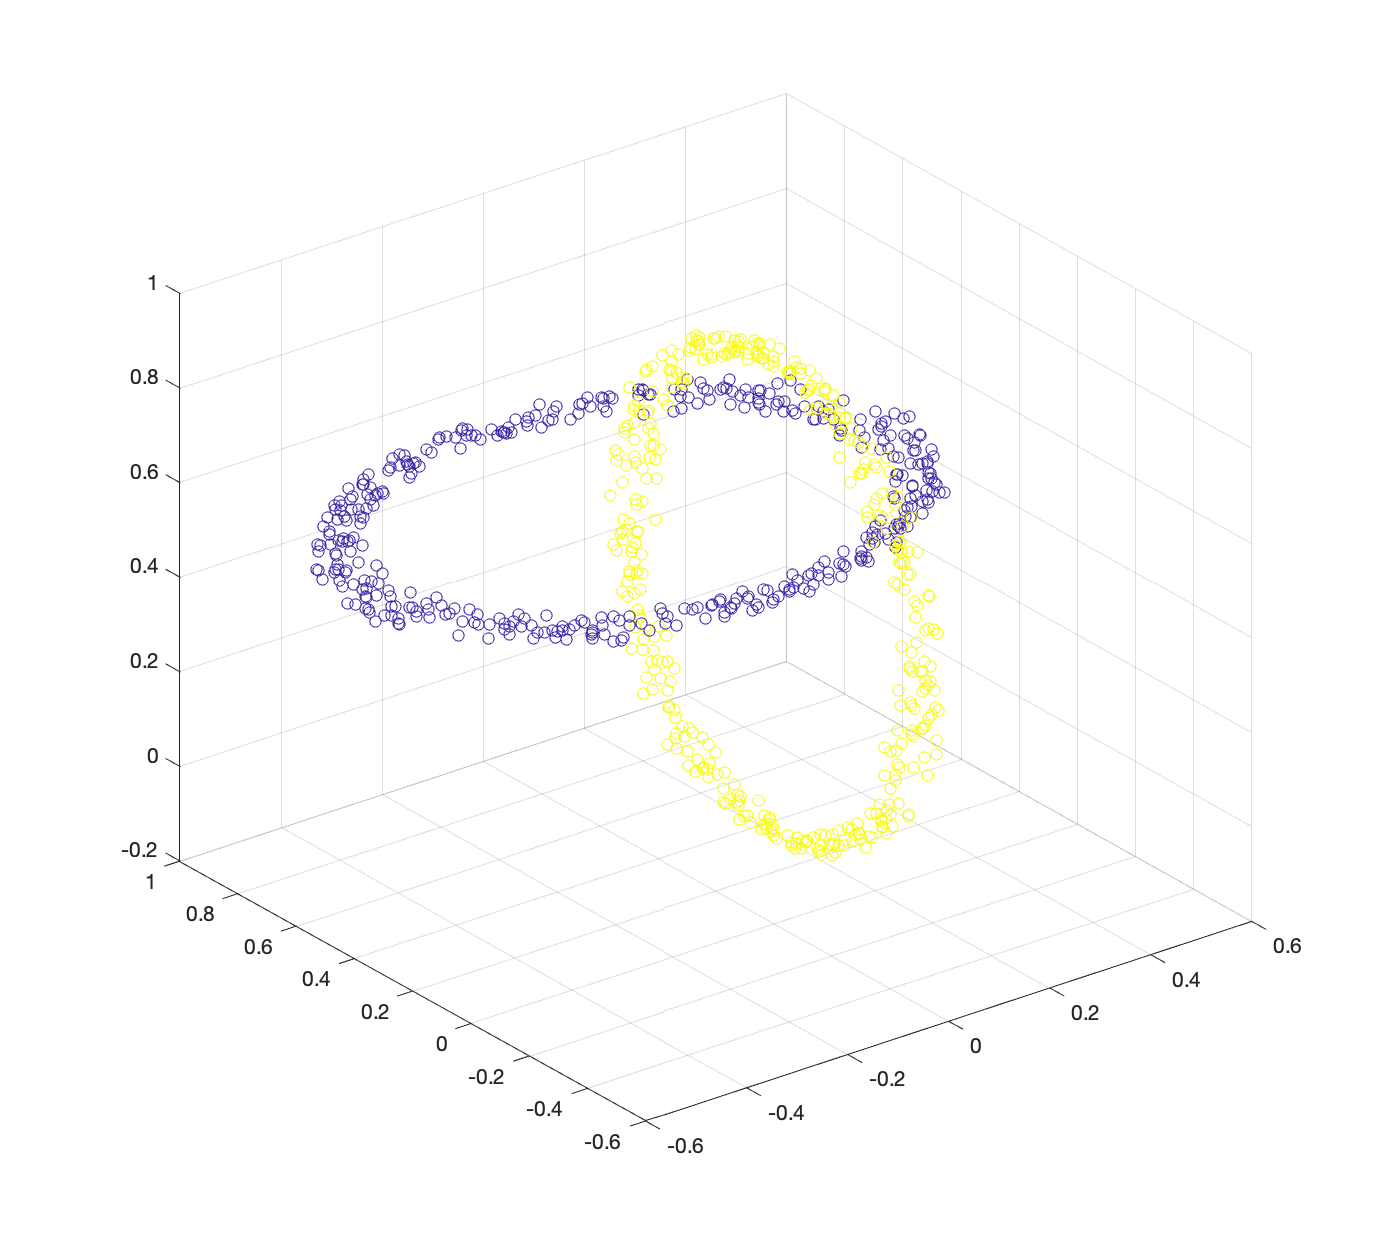
\includegraphics[width=0.45\textwidth]{../src/figures/spectral/rings_clusters_10}
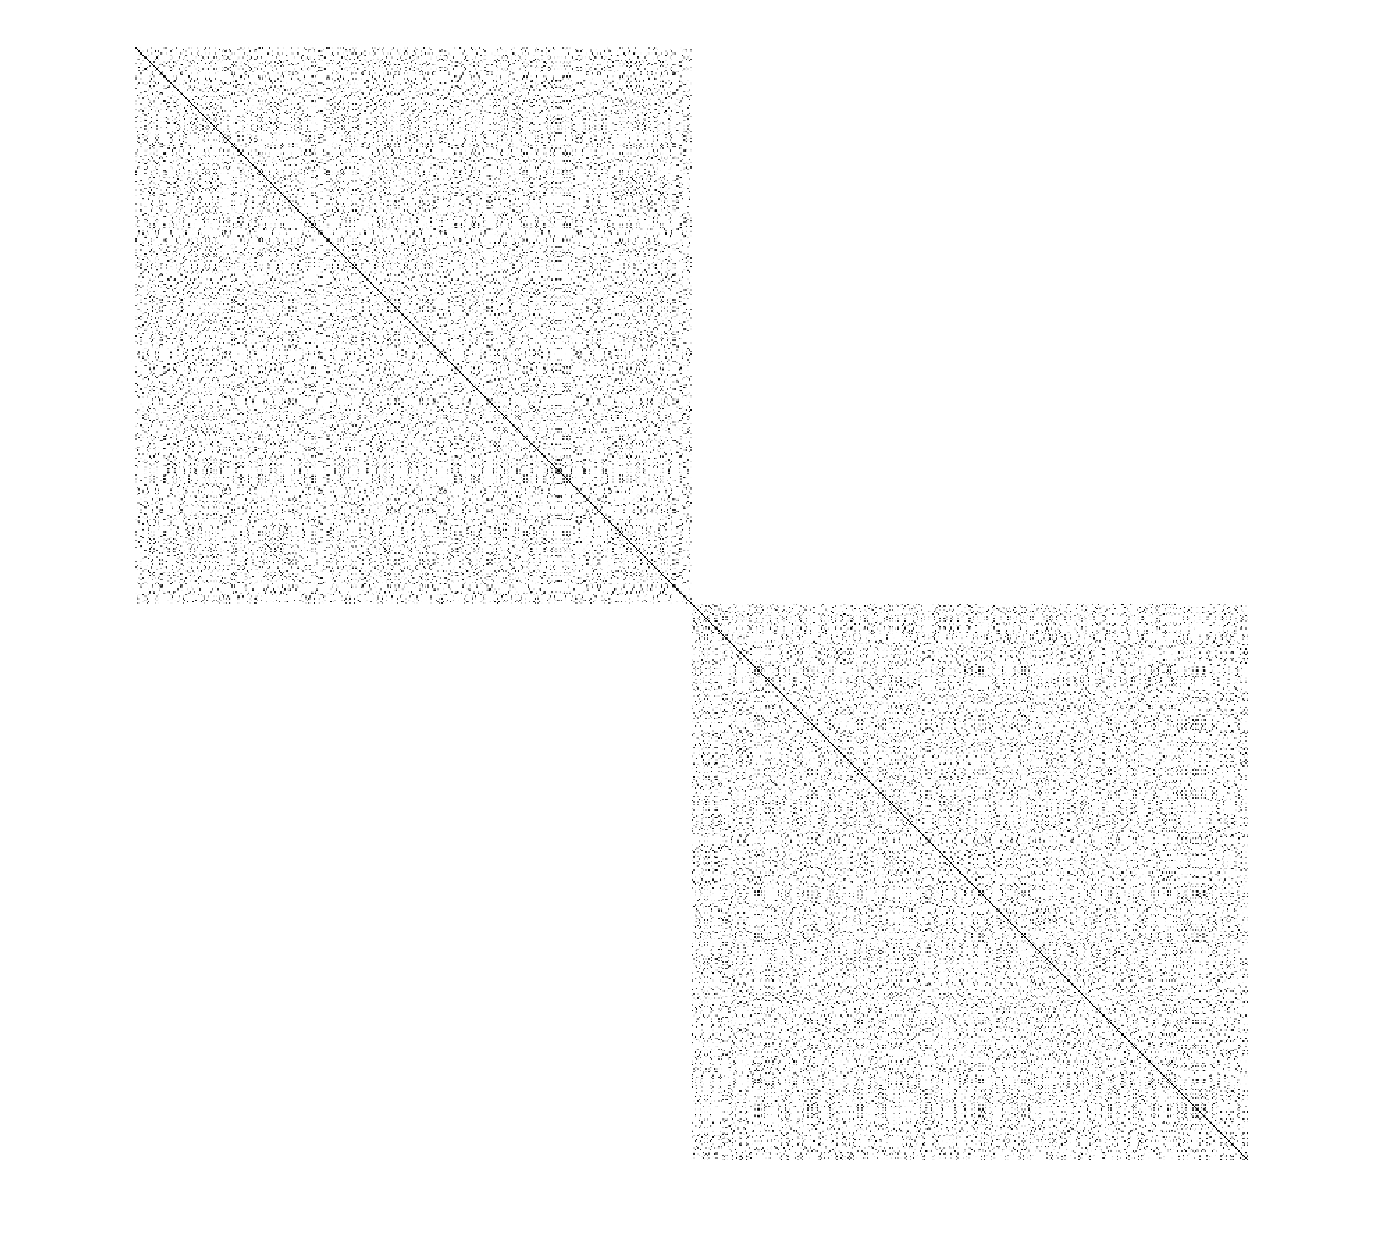
\includegraphics[width=0.4\textwidth]{../src/figures/spectral/rings_block_10}
\end{minipage}}\quad
\subfloat[$\sigma^2=1.0$.]{
\begin{minipage}{0.48\textwidth}
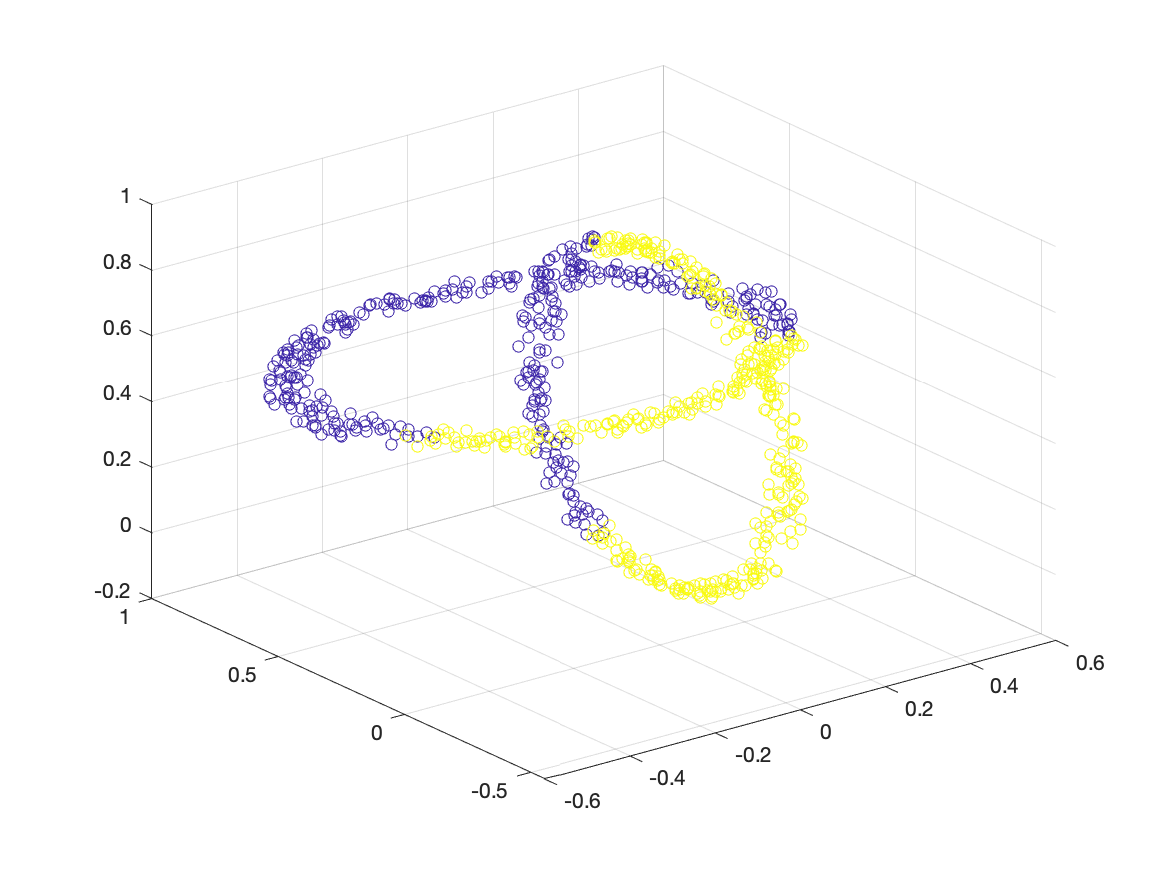
\includegraphics[width=0.45\textwidth]{../src/figures/spectral/rings_clusters_1000}
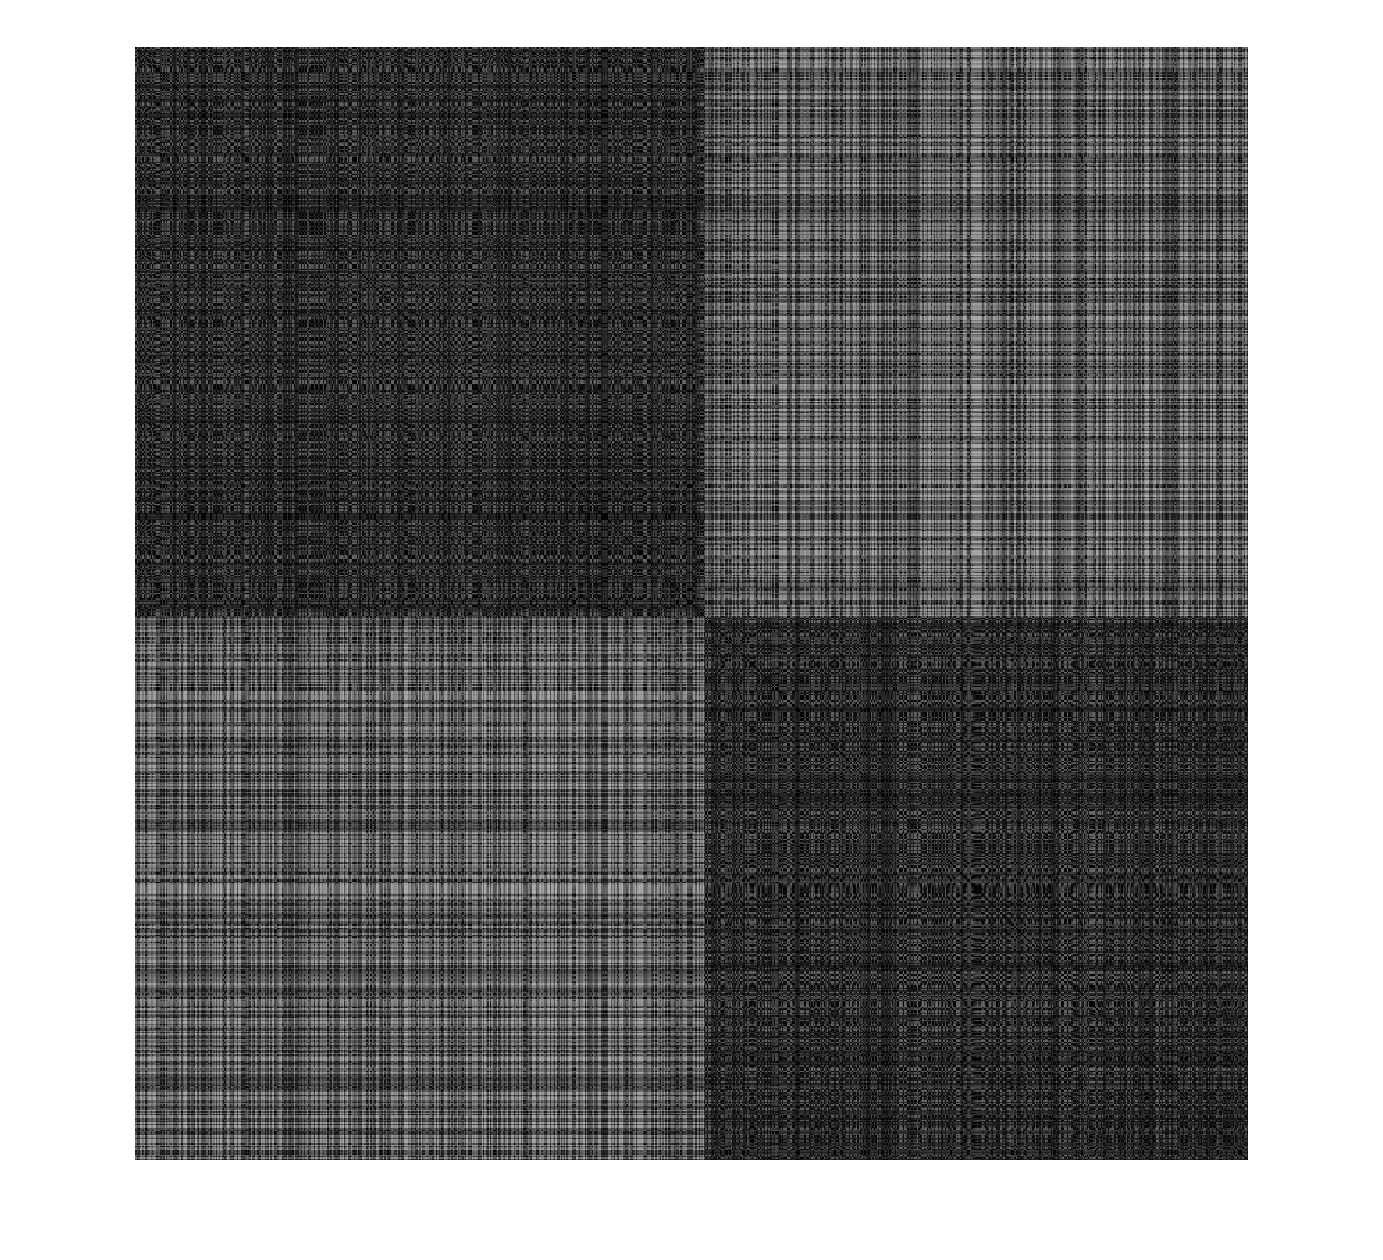
\includegraphics[width=0.4\textwidth]{../src/figures/spectral/rings_block_1000}
\end{minipage}}\\
%
\caption{Clustering of a toy dataset consisting of two rings. KSC applied using a kernel with varying $\sigma^2$ values. When this bandwidth is too large the reach of influence of each data point becomes too large and the clustering becomes subpar.}
\label{spectraltoy}
\end{figure}

\par Spectral clustering in particular deals with finding a minimal cut of a similarity graph (a weighted \& undirected graph) rather than finding a decision boundary which separates classes. Since finding a balanced yet minimal cut is NP-hard a relaxed version is considered instead. The solution of the relaxed version is based on the eigendecomposition of the Laplacian matrix of the graph such that the data points can be embedded in an eigenspace on which a clustering algorithm like \textit{k-means} can be applied. 

\begingroup
\setlength{\columnsep}{0.2cm}
\setlength{\intextsep}{0cm}
\begin{wrapfigure}{r}{.3\textwidth}
\vspace{-0.6cm}
\begin{minipage}{\linewidth}
    \centering\captionsetup[subfigure]{justification=centering}
    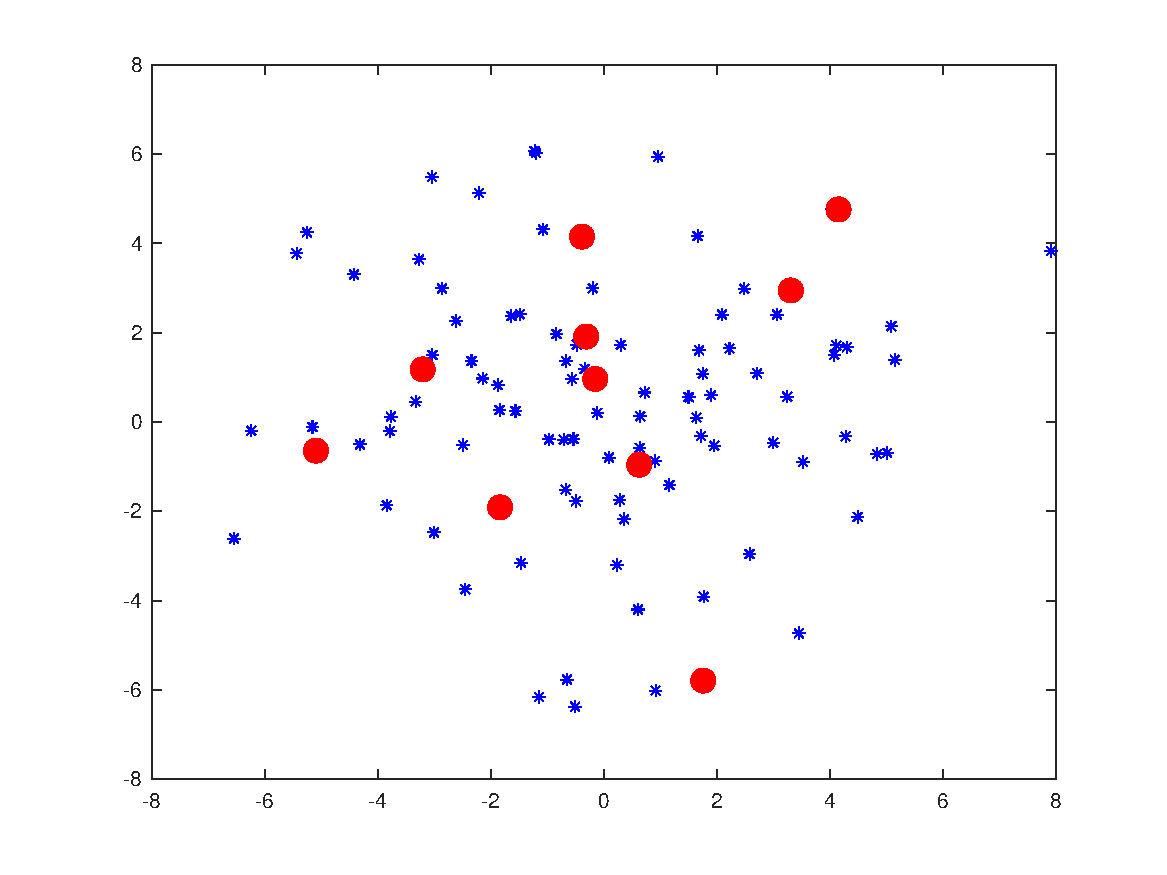
\includegraphics[width=\linewidth]{../src/figures/fixedsize/fixedsize_1}
    \caption*{$\sigma^2=0.01$}
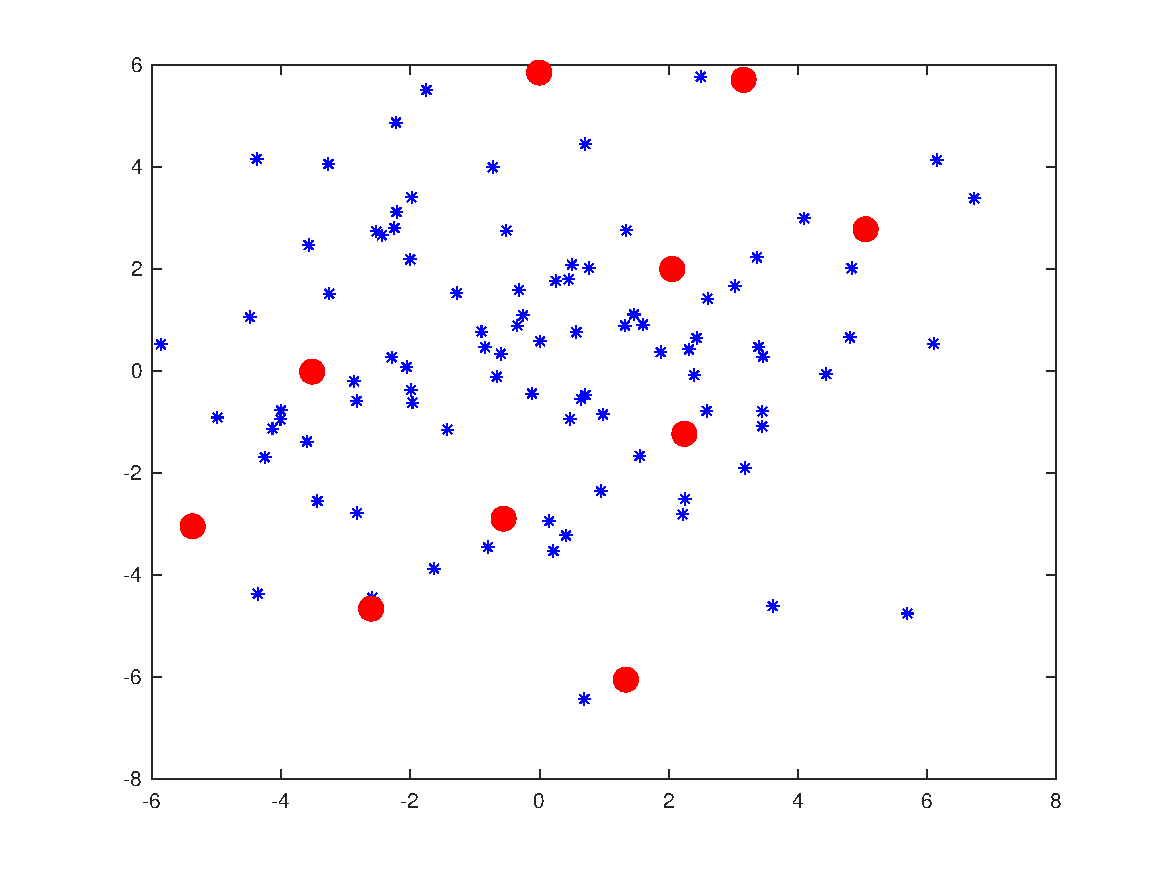
\includegraphics[width=\linewidth]{../src/figures/fixedsize/fixedsize_10}
    \caption*{$\sigma^2=0.1$}
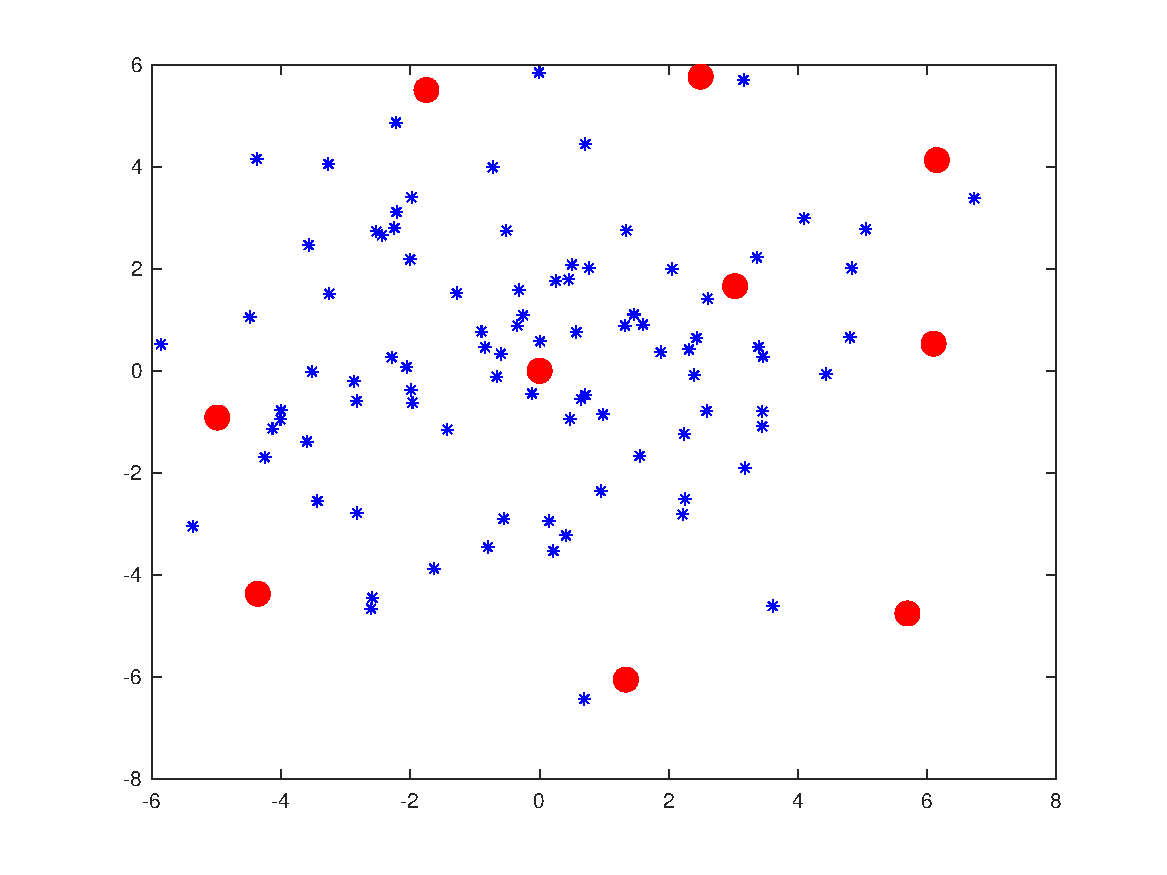
\includegraphics[width=\linewidth]{../src/figures/fixedsize/fixedsize_100}
    \caption*{$\sigma^2=1.0$}
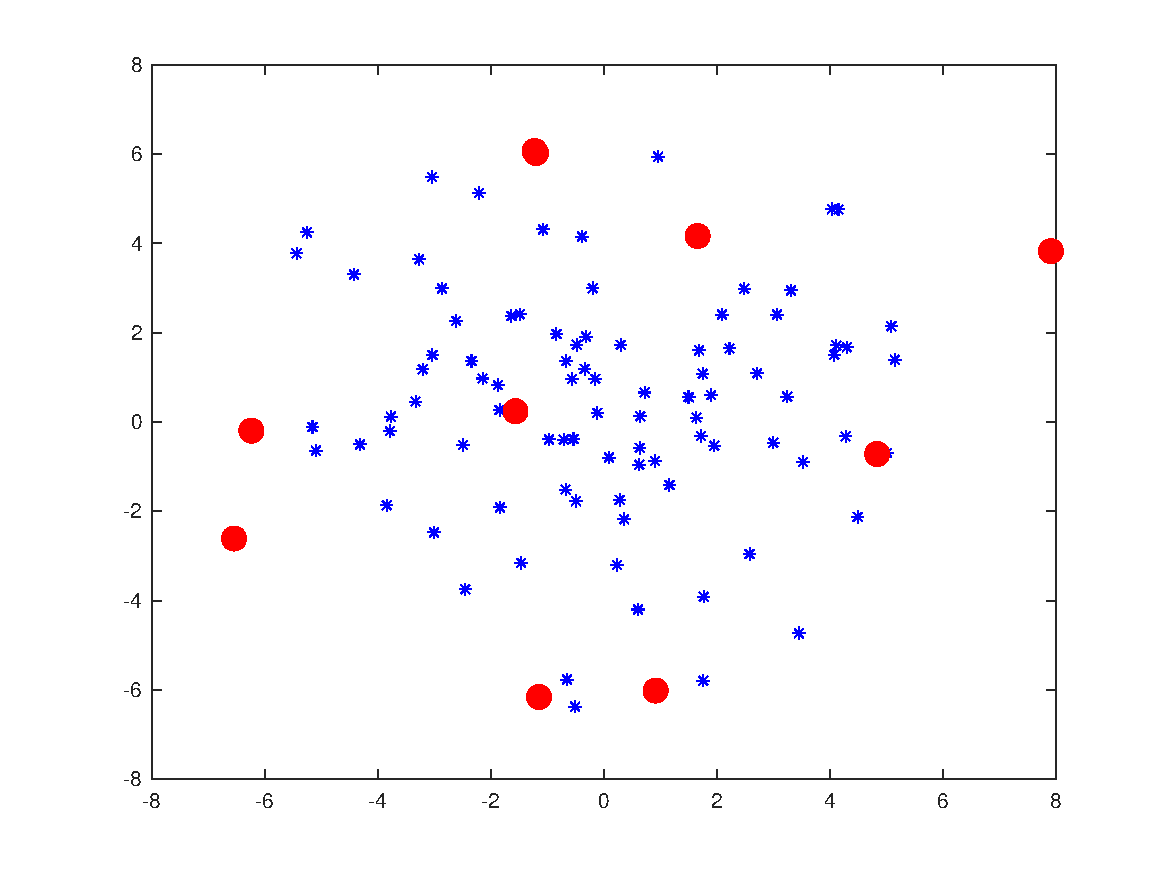
\includegraphics[width=\linewidth]{../src/figures/fixedsize/fixedsize_1000}
    \caption*{$\sigma^2=10.0$}
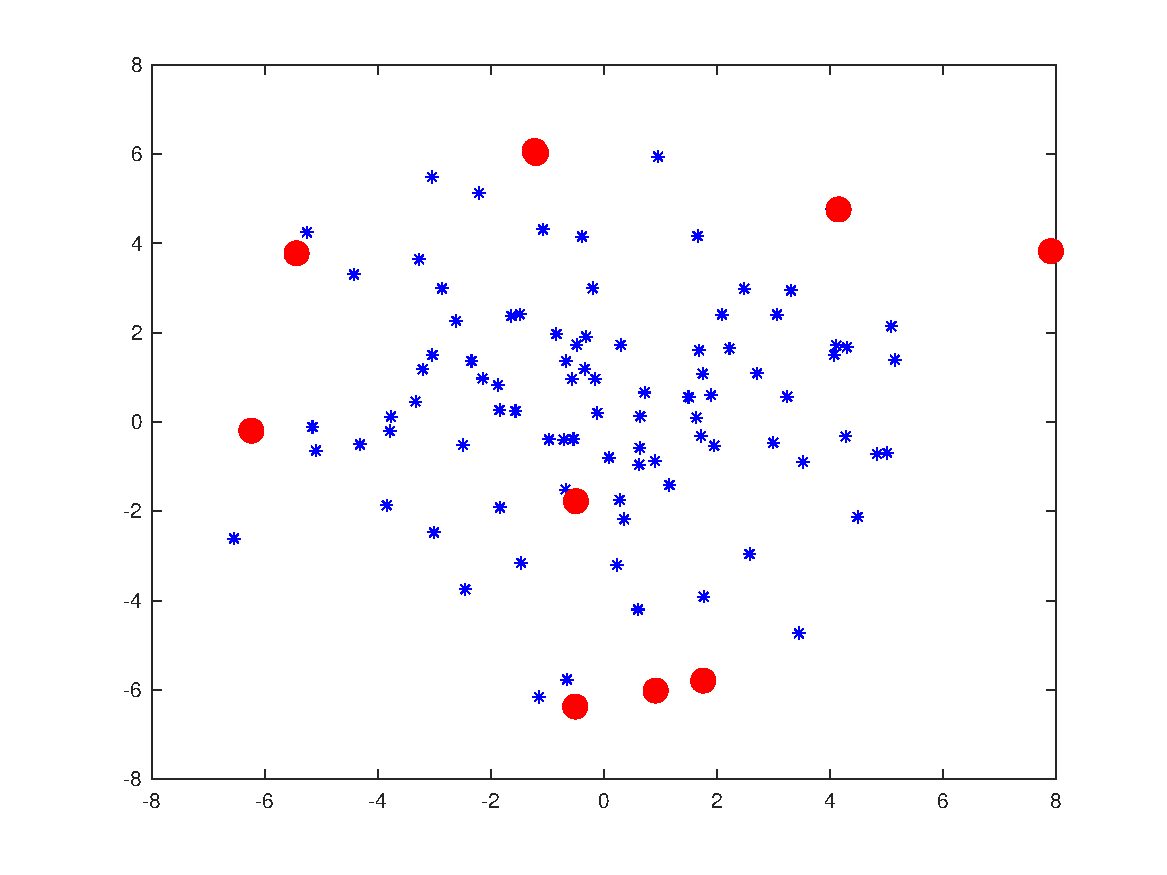
\includegraphics[width=\linewidth]{../src/figures/fixedsize/fixedsize_10000}
    \caption*{$\sigma^2=100.0$}
\end{minipage}
\caption{Subsample of input data points obtained for a fixed-sized LS-SVM using an RBF kernel of varying $\sigma^2$.}
\label{fixedsample}
\end{wrapfigure}

\par The Laplacian matrix captures a lot of information about the graph such as the number of connected components (which equals the multiplicity of the eigenvalue $\lambda=0$). Related to this number is the property that if the data is sorted according to cluster membership the similarity matrix becomes block-diagonal. Such depictions are used in the figures above. 

\par \textit{Kernel spectral clustering (KSC)} reformulates spectral clustering as an LS-SVM, essentially boiling down to a weighted version of kernel PCA. Again, out-of-sample extensions become possible and one can apply it on large-scale problems. 

\par Experiments with an RBF kernel are shown in figure \ref{spectraltoy}. Since the similarity matrix is the Kernel function and $\sigma^2$ happens to control the contrast in similarity between data points a $\sigma^2$ value which is small leads to a single class as all points are considered similar while a larger $\sigma^2$ leads to poor clustering results.

\fakesubsection{Fixed-size LS-SVM}{}

Sometimes the amount of data that is being dealt with is too large such that some of the matrices like the kernel matrix involved in the dual formulations cannot be stored in memory. It becomes desirable, then, to solve the problem in the primal rather than in the dual space (it's the other way round when the number of input dimensions is high). The problem with this is that the feature map $\phi(x)$ is generally not known, only the kernel function representing dot products is made explicit.

\par While decomposition can be used for this an approach that can be considered in the case of fixed-size LS-SVMs is the Nystr\"om method which is traditionally used for integral approximation. In the current setting it means that one takes a random subsample of the input data (of size $M\ll N$) and then uses this to approximate the feature map $\phi(x)$ such that a parametric solution can be found. For fixed-size LS-SVMs the subsample starts randomly and is then updated iteratively as long as the Renyi entropy improves. This metric can be approximated by taking the sum of the elements of the kernel.

\par Examples of subsamples obtained through optimisation of the Renyi entropy are shown in figure \ref{fixedsample}. The kernel is a Gaussian one, the input data is normally distributed. It looks as though a larger value for $\sigma^2$ leads to a selection of data points that are more spread out.

\par In figure \ref{fscomp} a fixed-size LS-SVM approach is compared with a variant which applies an $\ell_0$-penalty after generating a fixed-size LS-SVM solution. This post-processing does not influence the total runtime because its complexity is $\mathcal{O}(M^3)$ while that of the fixed-size LS-SVM is $\mathcal{O}(NM^2)$. While the error increases the number of support vector is much lower for the latter method. This is not surprising since the $\ell_0$-norm counts the number of non-zero values which means that it aims for sparse representations. The error drops as well, presumably because the model generalises better.

\endgroup

\begin{figure}[h]
\centering
%
\subfloat[Error estimation.]{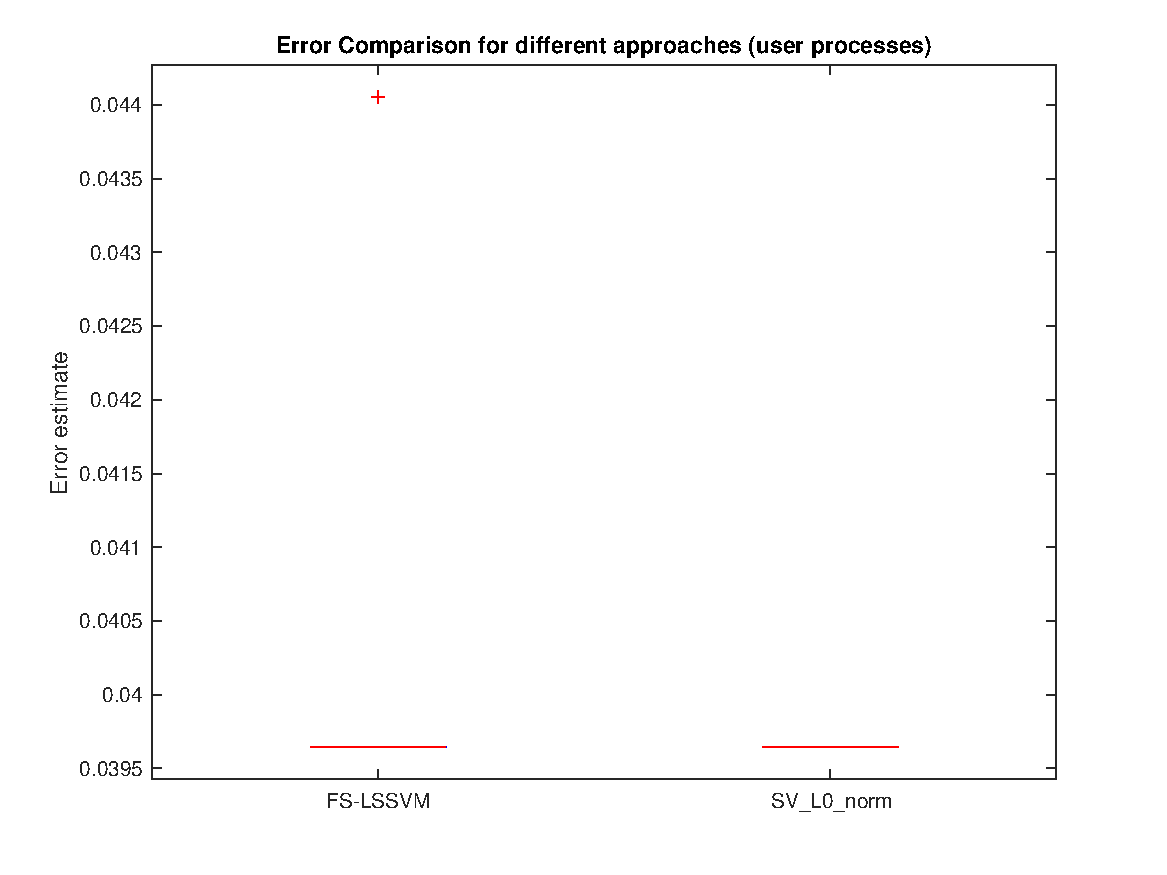
\includegraphics[width=0.25\textwidth]{../src/figures/fixedsize/comparison_error}}\quad
\subfloat[Number of support vectors.]{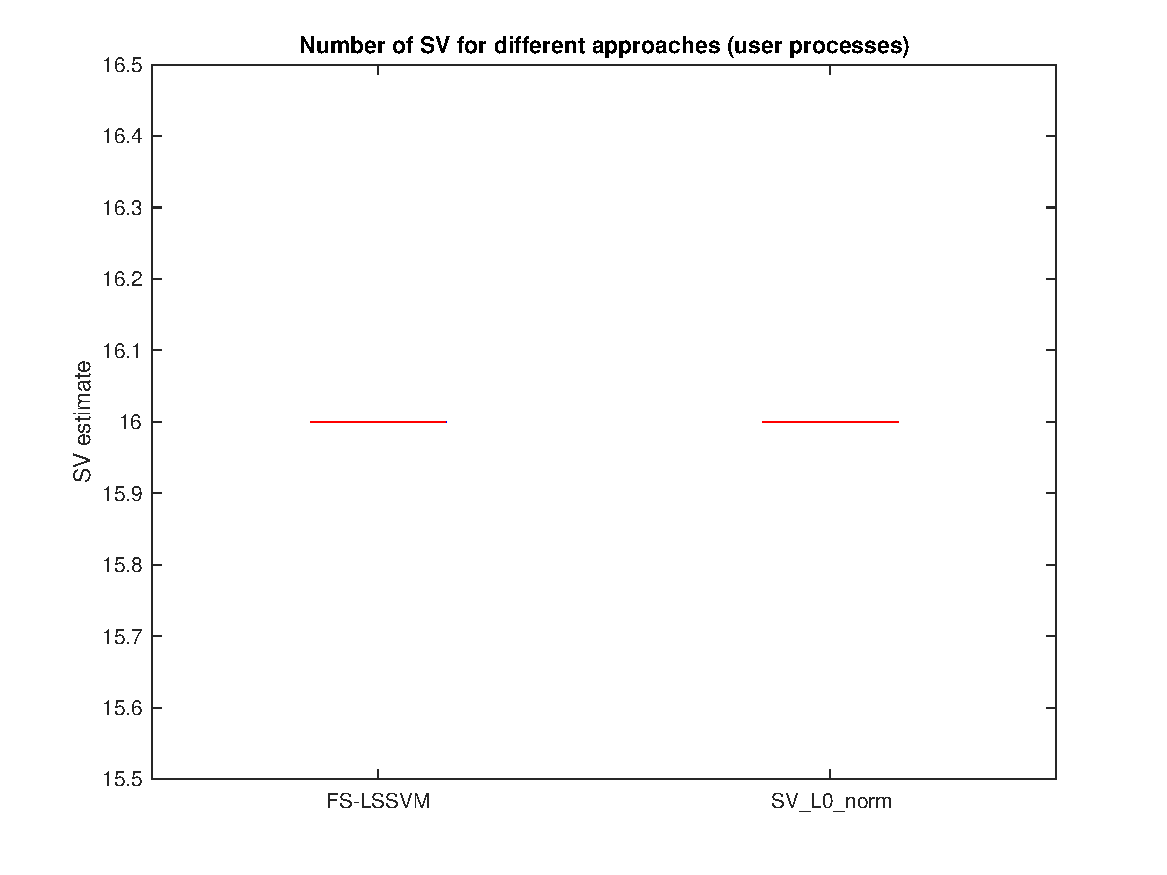
\includegraphics[width=0.25\textwidth]{../src/figures/fixedsize/comparison_sv}}\quad
\subfloat[Time taken for generating the models.]{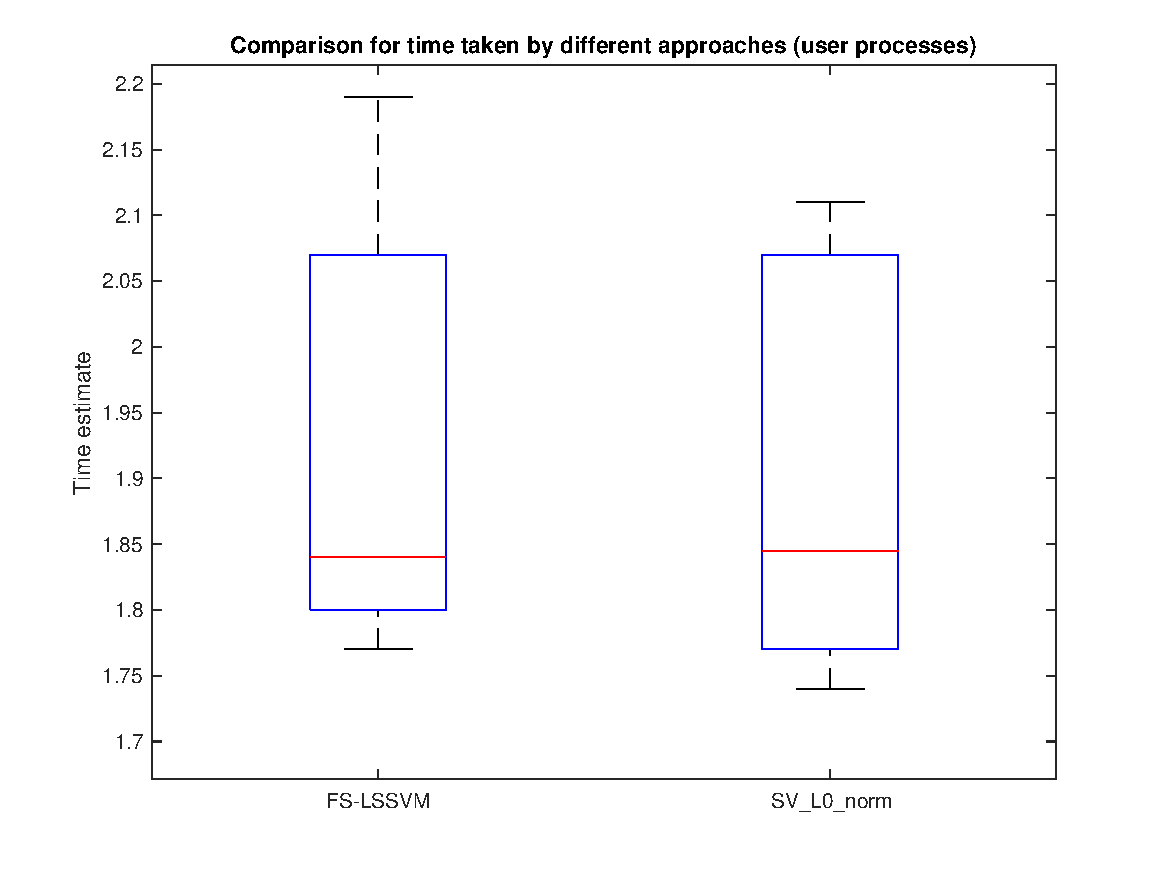
\includegraphics[width=0.25\textwidth]{../src/figures/fixedsize/comparison_time}}\\
%
\caption{Comparison of the standard fixed-size LS-SVM approach with a modified approach applying an $\ell_0$-penalty to obtain a sparser representation.}
\label{fscomp}
\end{figure}

\fakesubsection{Kernel principal component analysis}{}


\fakesubsection{Fixed-size LS-SVM}{}

